In questo capitolo verranno mostrati degli esperimenti per valutare il funzionamento e le prestazioni del sensore. 
Per l'analisi della \textbf{reattivit\'{a}}, viene osservato il comportamento del sensore nel caso in cui ci sia 
un cambiamento istantaneo delle forze in gioco. 
Un'altro importante aspetto da valutare \'{e} la \textbf{precisione} dei dati forniti dal sensore. Per farlo 
si \'{e} pensato di utilizzare le misurazioni effettuate per calcolare la viscosit\'{a} di un liquido di cui se ne conosce 
il valore. 
Prima di mostrare i risultati di questi due esperimenti \'{e} bene, per\'{o}, parlare dell'importanza dell'azzeramento periodico 
del sensore.

\section{Errore nelle misurazioni}
Come spiegato nel Capitolo \ref{chapter:chapter2}, il sensore \`{e} soggetto a rumore di fondo intrinseco che 
pu\`{o} essere causato da diversi fattori, come la temperatura, l'instabilit\`{a} dell'alimentazione o il rumore elettrico. 
\newpage
\begin{figure}[H]
    \centering
    \includegraphics*[width=0.80\textwidth]{images/drifting.png}
    \caption{Drifting lungo l'asse z}
    \label{fig:drifting}
\end{figure}
In Figura \ref{fig:drifting} viene mostrato il fenomeno del \textbf{drifting}: ossia quando un sensore nel corso del tempo 
mostra una deviazione nelle sue letture senza un'effettiva variazione delle condizioni ambientali. Questo fenomeno si verifica 
solamente se il sensore viene collegato al PC come indicato nella Sezione \ref{sec:scp}. 
Si pu\`{o} notare come la forza rilevata dal sensore lungo l'asse z decresca per i primi 250 secondi, per poi 
cominciare una fase di crescita lineare senza che al sensore venga applicata alcuna forza. 
La forza misurata supera la soglia di confidenza specificata nel manuale entro la 
quale la misurazione deve essere catalogata come non attendibile. 
Per ovviare a questo problema, nel caso in cui si optasse per un collegamento passante per la control box del robot, 
sarebbe necessario azzerare il sensore periodicamente in modo che le letture risultino corrette e senza deviazioni. 
Gli esperimenti descritti nel corso di questo capitolo e le applicazioni presenti nel Capitolo \ref{chapter:chapter5}, sono state 
sviluppate utilizzando un collegamento diretto tra sensore e PC via USB.


\section{Taglio del filo}
Al fine di valutare la reattivit\`{a} del sensore coppia-forza, \`{e} stato condotto un esperimento per esaminare la capacit\`{a} del 
sensore di rilevare rapidamente una variazione istantanea della forza. 
Tale variazione improvvisa \`{e} stata simulata 
tagliando un filo che sosteneva un oggetto appeso al sensore. La misurazione rilevata a seguito del taglio  
deve mostrare una variazione \textbf{proporzionale al peso dell'oggetto}.
In questo esperimento, \`{e} stato attaccato al sensore un filo con appeso un oggetto di 0.155 Kg. 
Il braccio \`{e} stato posizionato in modo tale che la forza peso gravasse solo su un asse del sensore alla volta, cosicch\`{e} 
il valore rilevato dopo il taglio fosse compatibile con il peso dell'oggetto precedentemente attaccato. 
In Figura \ref{fig:setup_z}, viene mostrato il setup per l'esperimento lungo l'asse z. 
\newpage
\begin{figure}[H]
    \centering
    \begin{subfigure}[b]{0.4\textwidth}
        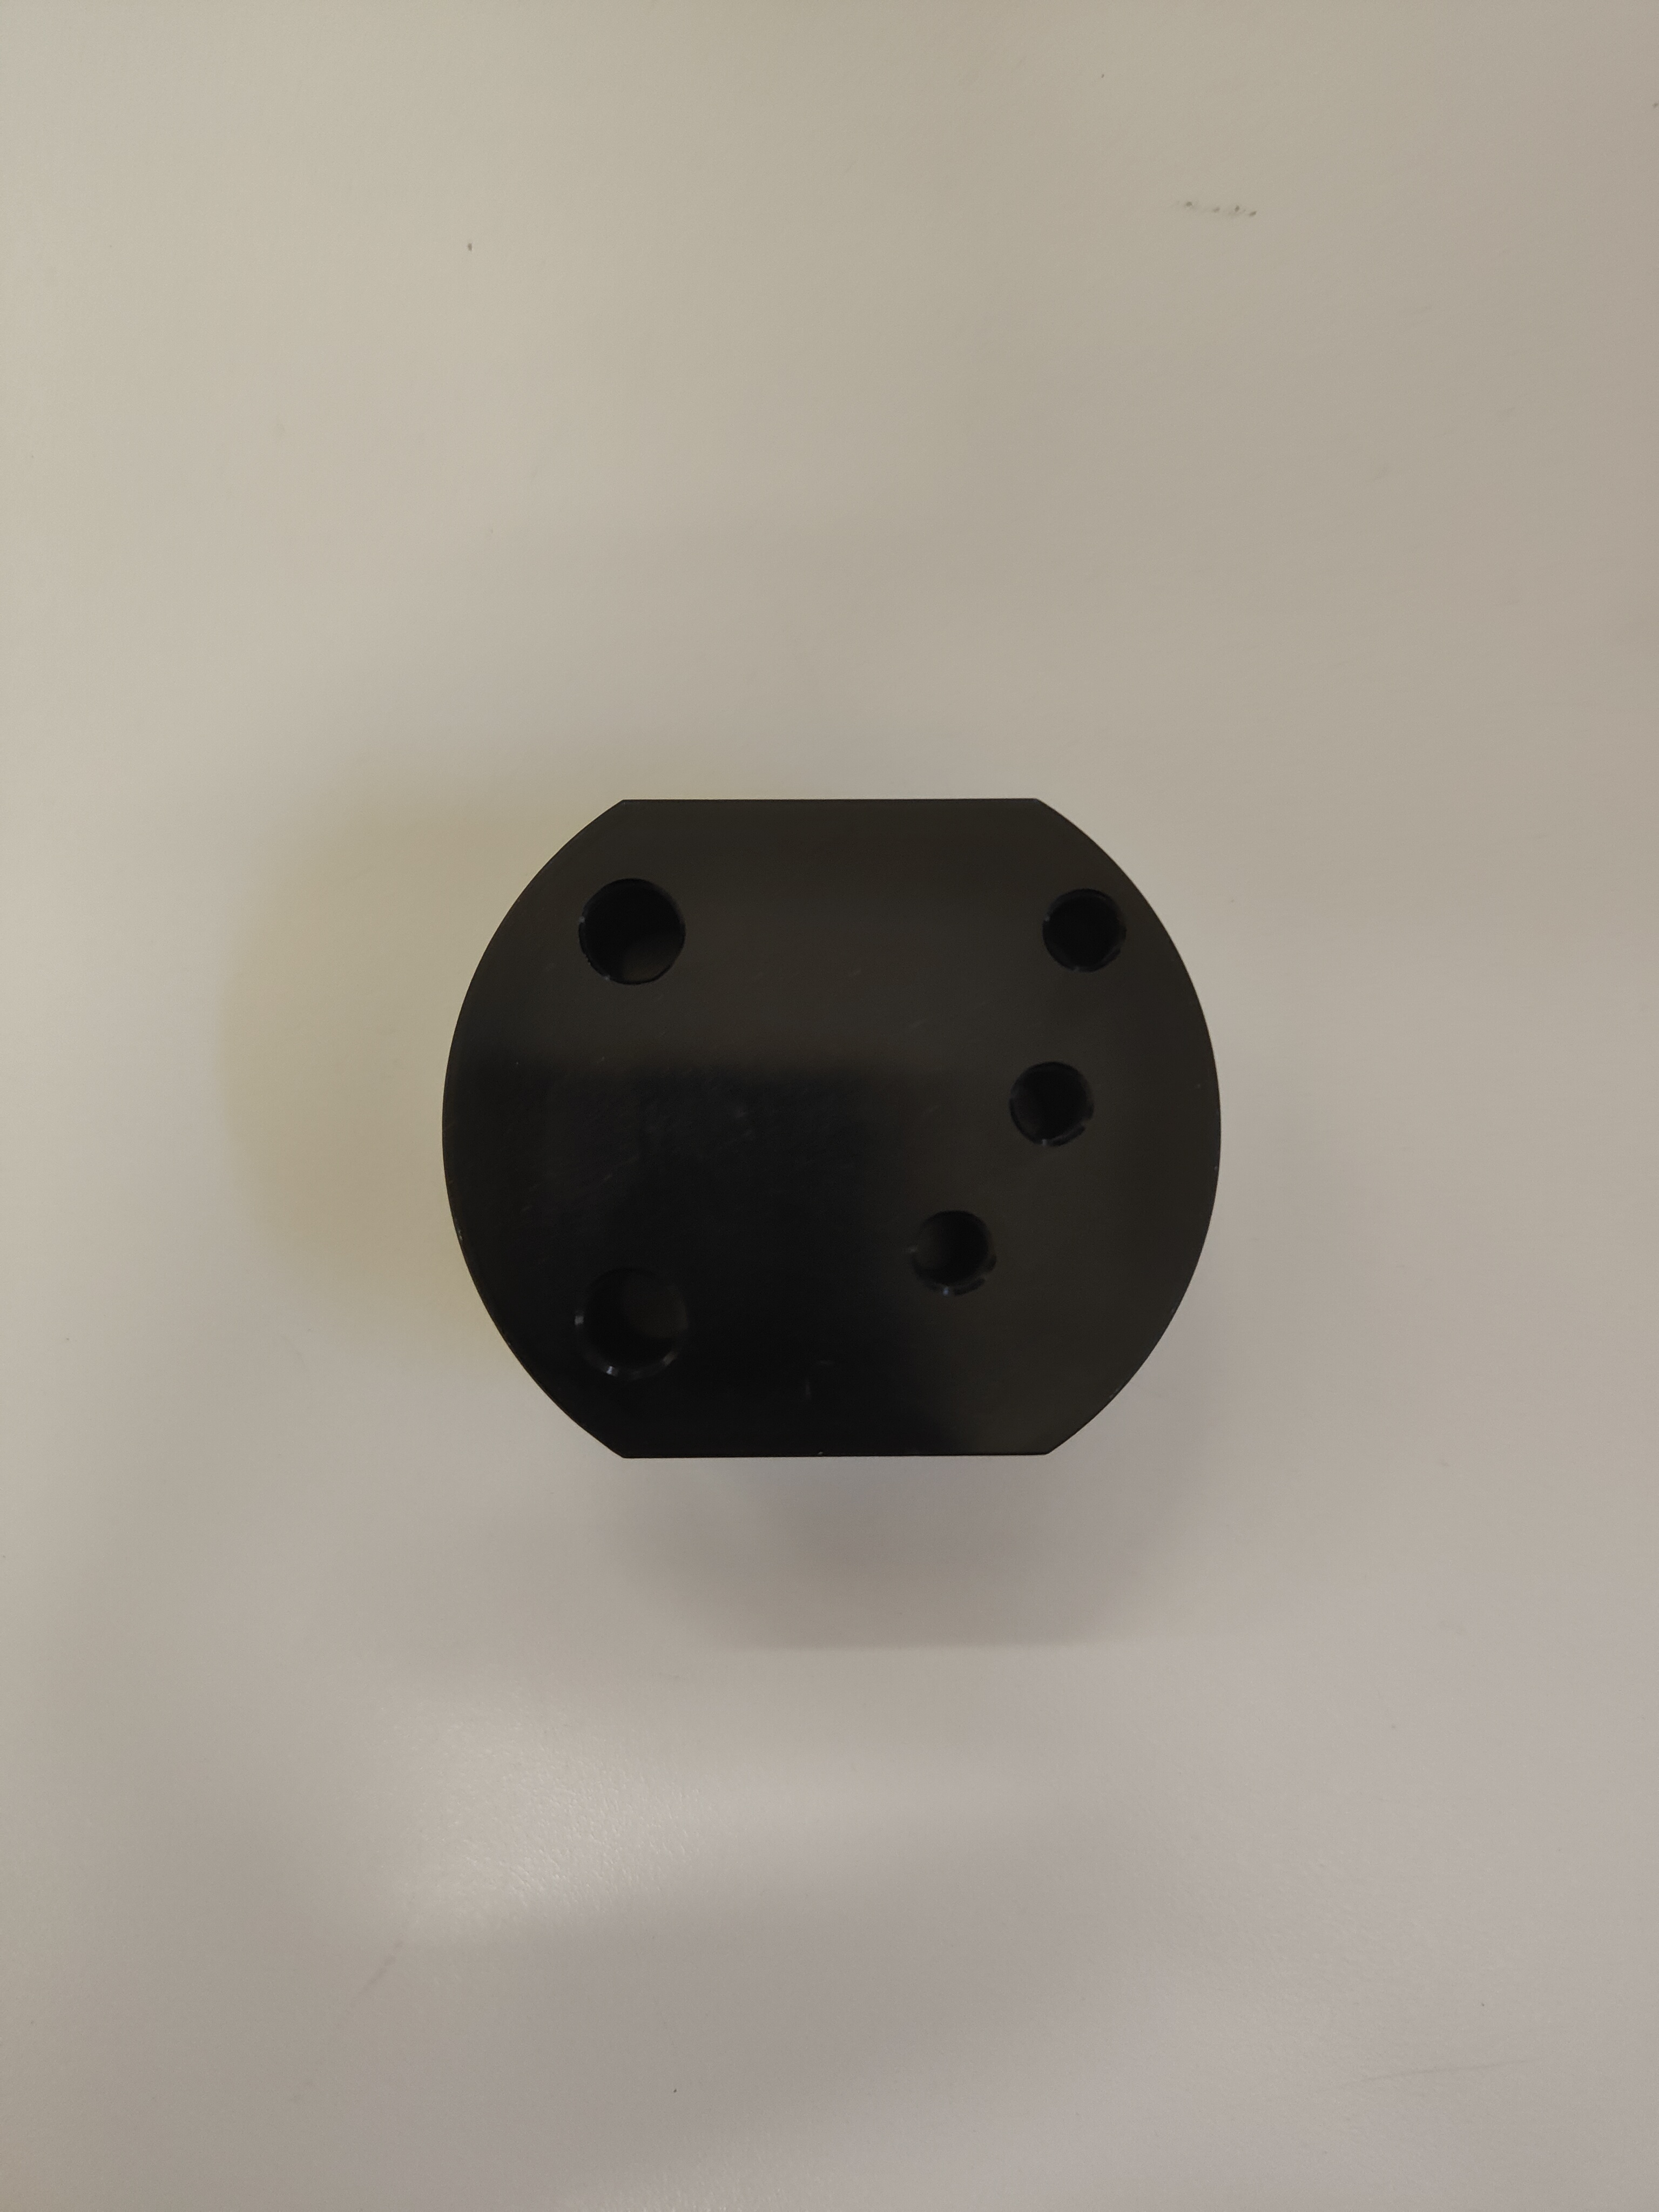
\includegraphics[width=\textwidth]{images/object.jpg}
        \label{fig:object}
    \end{subfigure}
    \qquad
    \begin{subfigure}[b]{0.4\textwidth}
        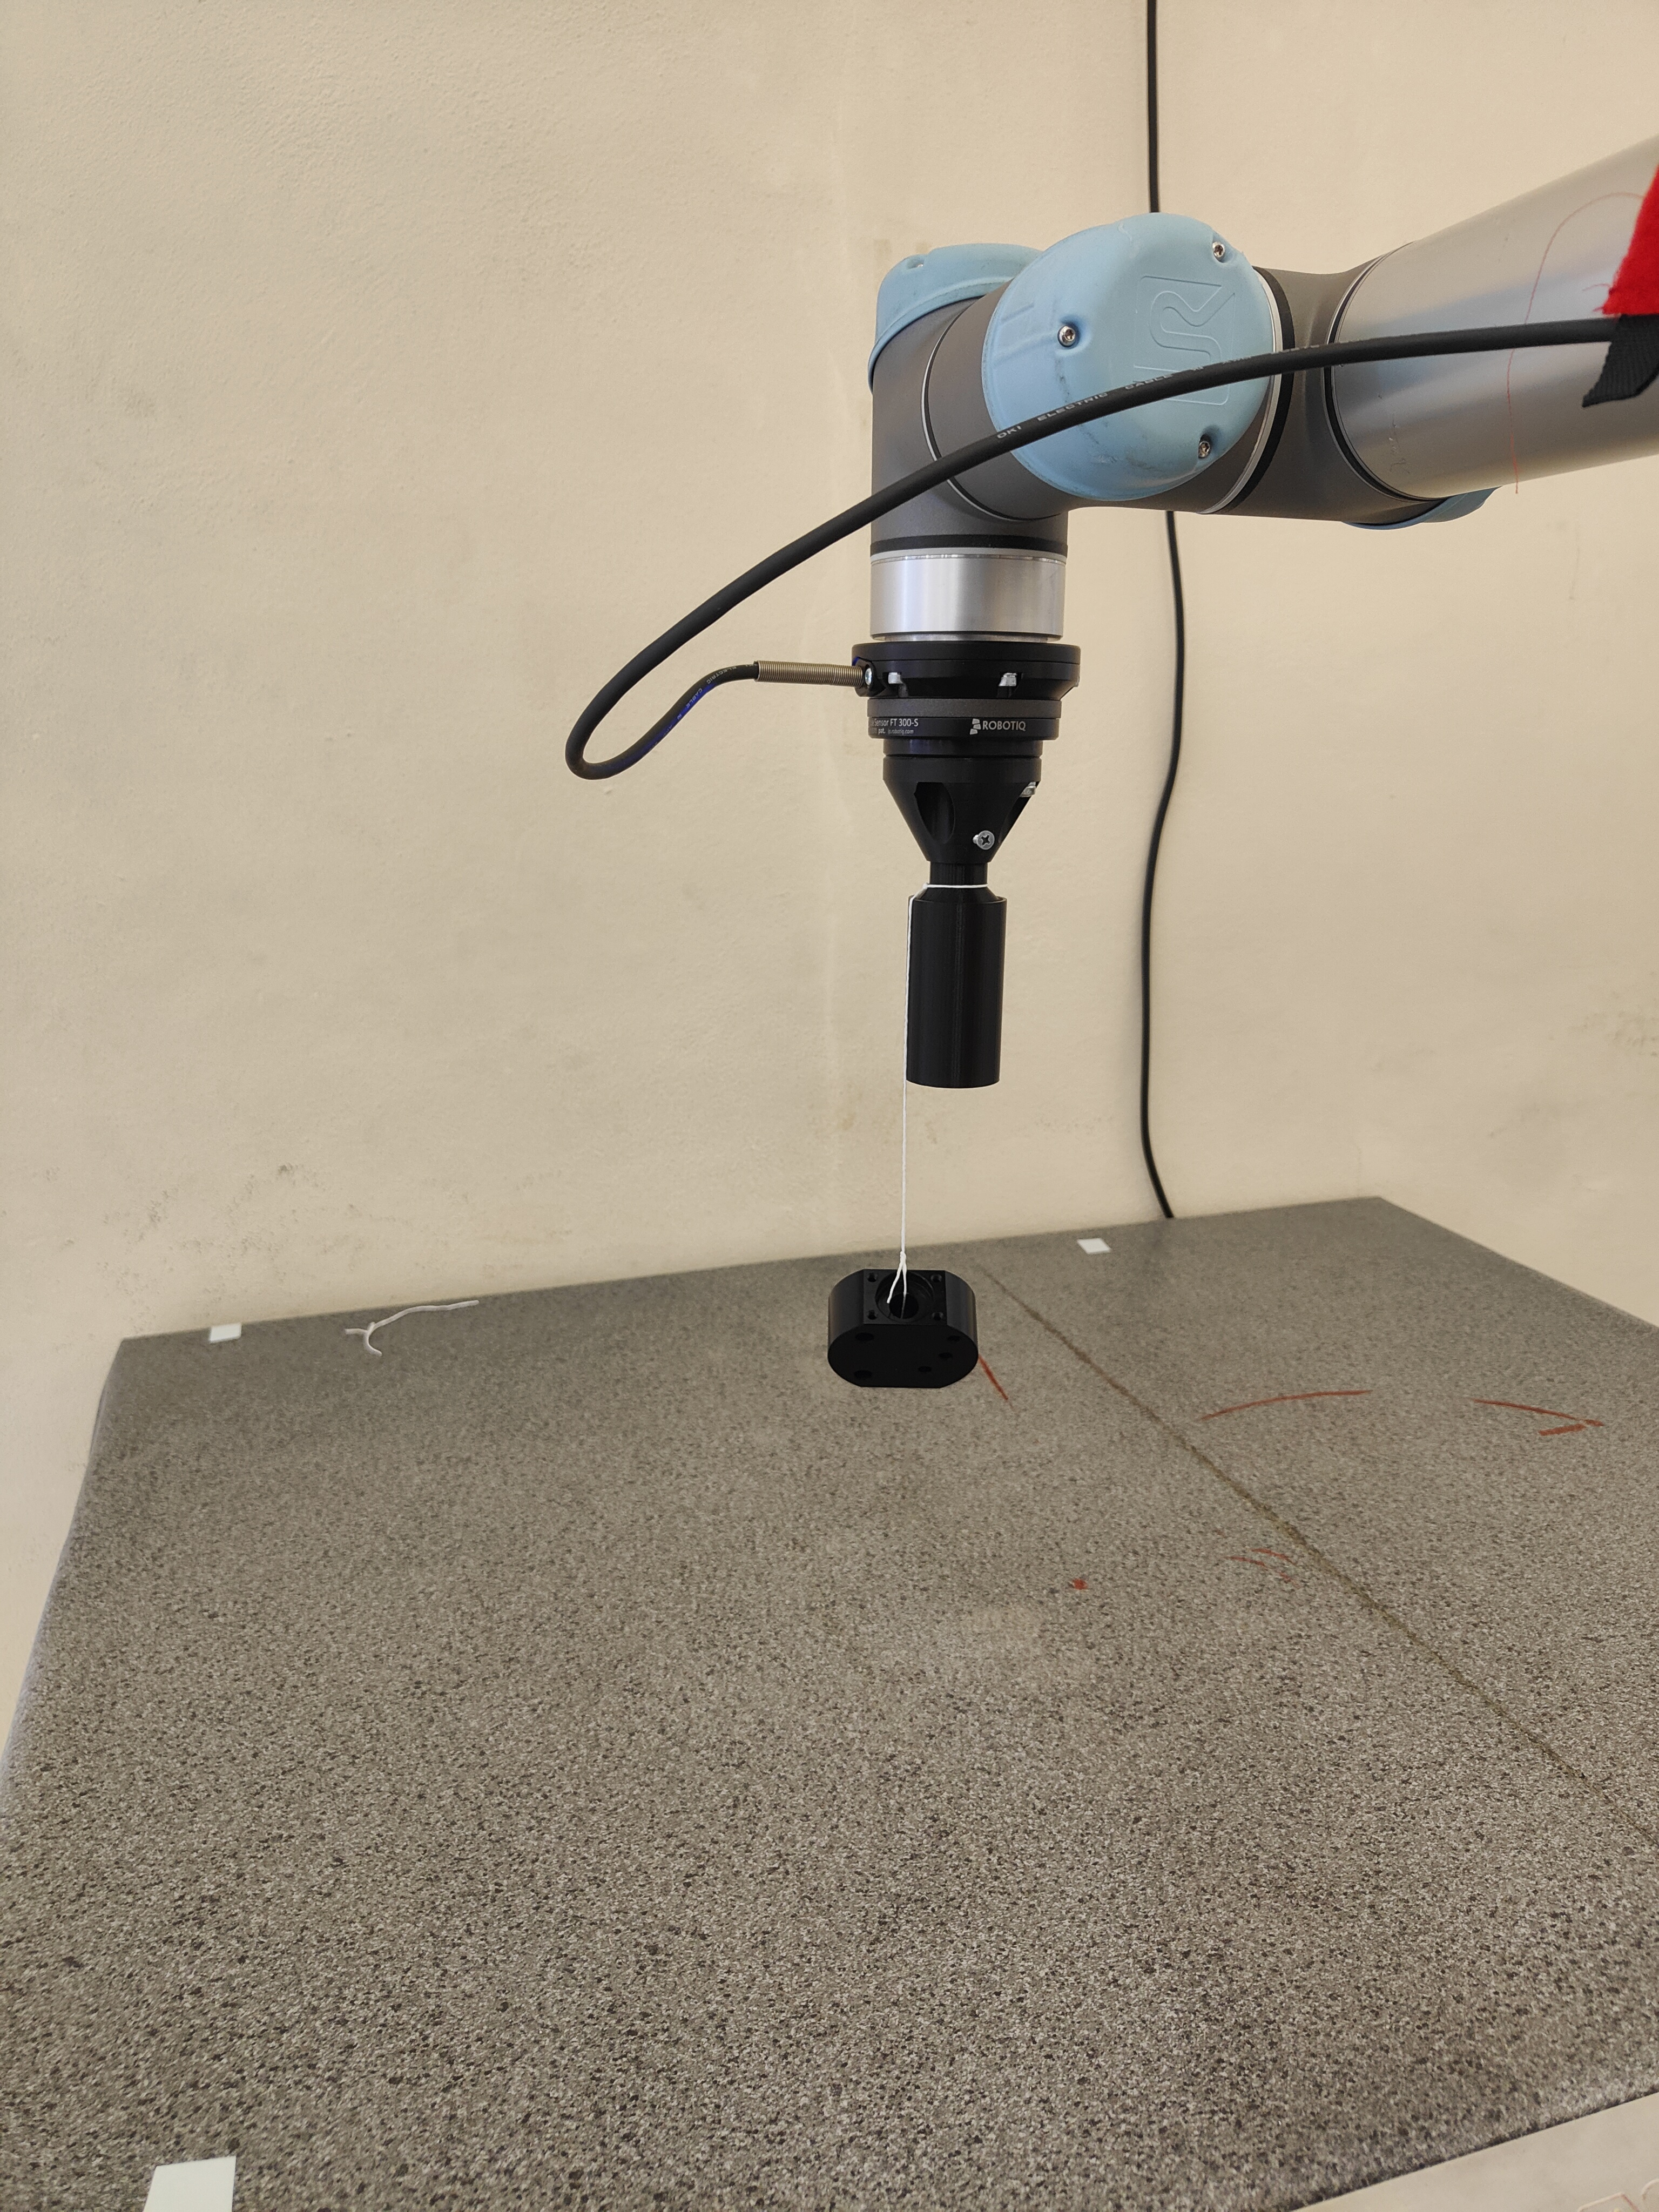
\includegraphics[width=\textwidth]{images/setup_z.jpg}
        \label{fig:setup}
    \end{subfigure}
    \caption{Setup sperimentale per l'analisi della reattivit\`{a}. A sinistra, l'oggetto di metallo utilizzato, 
    a destra l'oggetto collegato con un filo al robot (forza peso che grava sull'asse z del sensore)}\label{fig:setup_z}
\end{figure}
Dopo aver azzerato il sensore, per verificarne la reattivit\`{a}, il filo \`{e} stato tagliato di netto. 
Il taglio del filo \`{e} un ottimo modo per `simulare' un cambiamento di forza istantaneo.
\begin{figure}[H]
    \centering
    \includegraphics*[width=0.85\textwidth]{images/z_cut.png}
    \caption{Andamento taglio del filo misurato lungo l'asse z del sensore coppia-forza}
    \label{fig:z_cut}
\end{figure}
In Figura \ref{fig:z_cut} viene mostrato l'andamento della forza rilevata dal sensore lungo l'asse z. 
Si pu\`{o} notare che, fino a quando il filo \`{e} attaccato al sensore, la forza rilevata \`{e} circa zero. 
Questo perch\'{e} il sensore \`{e} stato azzerato quando l'oggetto era gi\`{a} stato appeso al sensore. 
Nel momento in cui avviene il taglio, il grafico si allinea istantaneamente al peso reale dell'oggetto, 
ossia circa 1.5 N (il valore previsto dovrebbe essere $0.155 \text{ Kg} \cdot 9.81 \frac{\text{N}}{\text{Kg}} = 1.52055 \text{ N}$).
Tale esperimento \`{e} stato ripetuto anche per gli altri due assi, confermando lo stesso valore indicativo di -1.5 N.
\begin{figure}[H]
    \centering
    \includegraphics*[width=0.45\textwidth]{images/setup_x.jpg}
    \caption{Setup sperimentale per l'analisi della reattivit\`{a} lungo l'asse x del sensore coppia-forza}
    \label{fig:setup_x}
\end{figure}
Muovendo il robot nella configurazione mostrata in Figura \ref{fig:setup_x}, la forza peso dell'oggetto grava univocamente sull'asse x 
del sensore. 
Ruotando l'end effector di 90° si ottiene il setup equivalente per l'asse y.
I risultati vengono mostrati in Figura \ref{fig:x_cut} e \ref{fig:y_cut}. 
\begin{figure}[H]
    \centering
    \includegraphics*[width=0.85\textwidth]{images/x_cut.png}
    \caption{Andamento taglio del filo misurato lungo l'asse x del sensore coppia-forza}
    \label{fig:x_cut}
\end{figure}
\begin{figure}[H]
    \centering
    \includegraphics*[width=0.85\textwidth]{images/y_cut.png}
    \caption{Andamento taglio del filo misurato lungo l'asse y del sensore coppia-forza}
    \label{fig:y_cut}
\end{figure}
A differenza di quanto riportato nei primi due grafici, l'andamento della forza rilevata lungo l'asse y, presenta un picco 
anomalo dovuto al taglio non sufficientemente netto del filo.


\section{Calcolo della viscosit\'{a}}
In questa sezione viene mostrato un esperimento per valutare la precisione delle misurazioni del sensore\footnotemark{}. 
Per farlo si \'{e} pensato di usare i momenti angolari misurati dal sensore per calcolare la \textbf{viscosit\'{a}} del burro 
d'arachidi e confrontarla con il valore ufficiale noto (150-250 $\text{Pa} \cdot \text{s}$). 
A tal proposito \'{e} stato installato sull'UR5 un cilindro (di raggio 2cm e altezza 7.5cm) come end effector. 
Si \'{e} scelto di utilizzare un tool con questa forma per agevolare la determinazione della formula dell'attrito viscoso agente 
in questo caso.
In Figura \ref{fig:peanut_butter} viene mostrato il setup per questo esperimento. 
\newpage
\begin{figure}[H]
    \centering
    \includegraphics*[width=0.45\textwidth]{images/setup_viscosity.jpg}
    \caption{Setup sperimentale per l'analisi della precisione, composto da un vasetto di burro d'arachidi e un tool 
    cilindrico stampato in 3D}
    \label{fig:peanut_butter}
\end{figure}
Il cilindro, una volta immerso nel burro di arachidi, viene fatto ruotare attorno al suo asse con velocit\'{a} angolare 
costante. Il sensore, rileva quindi un momento torcente lungo l'asse z corrispondente alla forza di attrito viscoso esercitata 
dal fluido sul cilindro in rotazione. \'{E} dunque possibile utilizzare tali valori per ricavare sperimentalmente 
la viscosit\'{a} del burro d'arachidi e confrontarla con i dati ufficiali noti. 
La formula per il calcolo dell'attrito viscoso \'{e} la seguente 
\begin{equation*}
    M = 2\pi \cdot \eta \cdot \frac{\omega \cdot h}{\Delta r} \cdot r_{1}^{3}
\end{equation*}
con 
\begin{itemize}
    \item $\eta$: viscosit\'{a} del fluido
    \item $\omega$: velocit\'{a} angolare di rotazione
    \item h: altezza del cilindro
    \item $r_{1}$: raggio del cilindro
    \item $r_{2}$: raggio del barattolo
    \item $\Delta r$: $r_{2} - r_{1}$
\end{itemize}
Si pu\'{o} quindi `ribaltare' tale formula per ricavare la viscosit\'{a} dalla forza di attrito misurata 
\begin{equation} \label{eq:eta}
    \eta = \frac{M \cdot \Delta r}{2\pi \cdot \omega \cdot h \cdot r_{1}^{3}}
\end{equation}
Utilizzando velocit\'{a} di rotazione e dimensioni del cilindro ridotte, la forza d'attrito rilevata dal sensore sar\'{a} in generale 
piccola. \'{E} stato necessario utilizzare un liquido con una viscosit\'{a} elevata, quale il burro d'arachidi, per condurre l'esperimento in modo tale 
che le misurazioni non fossero minori della sensibilit\'{a} del sensore. 
Con MoveIt il braccio viene prima posizionato in modo tale che il cilindro sia immerso all'interno del burro d'arachidi. 
Come indicato in \ref{eq:eta}, per calcolare la viscosit\'{a} del fluido \'{e} necessario conoscere 
la velocit\'{a} di rotazione del cilindro. Con un controllore di posizione, tale informazione non \'{e} accessibile. 
Pertanto \'{e} necessario passare ad un controllore di velocit\'{a} (quale \verb|twist_controller|) per poter manovrare il robot in 
termini di velocit\'{a} e non in termini di posizione. Essendo questa un'operazione effettuata anche in altre applicazioni (vedi  
Capitolo \ref{chapter:chapter4}), sono state create delle apposite funzioni per il cambio dei controllori nel file \verb|utils.cpp|. 
Il robot, quindi, comincia a far ruotare su se stesso il cilindro a velocit\'{a} costante ($0.8 \frac{\text{rad}}{\text{s}}$) mentre 
il sensore acquisisce i dati della forza d'attrito. 
Viene poi calcolata la media di tutte le misurazioni effettuate (600) e, tale valore, viene usato per calcolare la viscosit\'{a} 
del burro d'arachidi. 
Nella seguente tabella vengono riportati i risultati delle misurazioni effettuate (in ordine cronologico)
\begin{center}
    \begin{tabular}{ ||c|c|c|c|c|c|| } 
     \hline
     $M \left[N \cdot m\right]$ & $\Delta r \left[cm\right]$ & $\omega \left[\frac{rad}{s}\right]$ & $h \left[cm\right]$ & $r_{1} \left[cm\right]$ & $\eta \left[Pa \cdot s\right]$\\
     \hline\hline 
     0.037298 & 1.5 & 0.8 & 7.5 & 2 & 185.506634 \\ 
     0.033253 & 1.5 & 0.8 & 7.5 & 2 & 165.388578 \\ 
     0.030207 & 1.5 & 0.8 & 7.5 & 2 & 150.235578 \\ 
     0.030003 & 1.5 & 0.8 & 7.5 & 2 & 149.224396 \\ 
     0.029157 & 1.5 & 0.8 & 7.5 & 2 & 145.013306 \\ 
     0.028872 & 1.5 & 0.8 & 7.5 & 2 & 143.595900 \\ 
     \hline
    \end{tabular}
\end{center}
La viscosit\'{a} fluttua parecchio nelle diverse misurazioni. Questo perch\'{e} le caratteristiche fisiche del burro d'arachidi 
cambiano durante ogni esperimento (aumento della temperatura per via dello sfregamento). Per avere misurazioni pi\'{u} attendibili 
sarebbe stato necessario riportare il fluido in condizione di riposo al termine di ogni misurazione. Il risultato pi\'{u} affidabile 
\'{e} il primo, in quanto \'{e} stato effettuato quando le propriet\'{a} fisiche del burro d'arachidi non erano ancora 
state alterate.
In media, la viscosit\'{a} del burro d'arachidi \'{e} $\eta = 156.494065$ $\text{Pa} \cdot \text{s}$, che rientra nel range di 
valori noto specificato inizialmente. 
\footnotetext{\url{https://github.com/andreastocco01/ur5_ft_tasks/blob/main/src/viscosity.cpp}}